\documentclass[
  shownotes,
  xcolor={svgnames},
  hyperref={colorlinks,citecolor=DarkBlue,linkcolor=DarkRed,urlcolor=DarkBlue}
  , aspectratio=169]{beamer}
\usepackage{animate}
\usepackage{amsmath}
\usepackage{amsfonts}
\usepackage{amssymb}
\usepackage{pifont}
\usepackage{mathpazo}
%\usepackage{xcolor}
\usepackage{multimedia}
\usepackage{fancybox}
\usepackage[para]{threeparttable}
\usepackage{multirow}
\setcounter{MaxMatrixCols}{30}
\usepackage{subcaption}
\usepackage{graphicx}
\usepackage{lscape}
\usepackage[compatibility=false,font=small]{caption}
\usepackage{booktabs}
\usepackage{ragged2e}
\usepackage{chronosys}
\usepackage{appendixnumberbeamer}
\usepackage{animate}
\setbeamertemplate{caption}[numbered]
\usepackage{color}
%\usepackage{times}
\usepackage{tikz}
\usepackage{comment} %to comment
%% BibTeX settings
\usepackage{natbib}
\bibliographystyle{apalike}
\bibpunct{(}{)}{,}{a}{,}{,}
\setbeamertemplate{bibliography item}{[\theenumiv]}

% Defines columns for bespoke tables
\usepackage{array}
\newcolumntype{L}[1]{>{\raggedright\let\newline\\\arraybackslash\hspace{0pt}}m{#1}}
\newcolumntype{C}[1]{>{\centering\let\newline\\\arraybackslash\hspace{0pt}}m{#1}}
\newcolumntype{R}[1]{>{\raggedleft\let\newline\\\arraybackslash\hspace{0pt}}m{#1}}


\usepackage{xfrac}


\usepackage{multicol}
\setlength{\columnsep}{0.5cm}

% Theme and colors
\usetheme{Boadilla}

% I use steel blue and a custom color palette. This defines it.
\definecolor{andesred}{HTML}{af2433}

% Other options
\providecommand{\U}[1]{\protect\rule{.1in}{.1in}}
\usefonttheme{serif}
\setbeamertemplate{itemize items}[default]
\setbeamertemplate{enumerate items}[square]
\setbeamertemplate{section in toc}[circle]

\makeatletter

\definecolor{mybackground}{HTML}{82CAFA}
\definecolor{myforeground}{HTML}{0000A0}

\setbeamercolor{normal text}{fg=black,bg=white}
\setbeamercolor{alerted text}{fg=red}
\setbeamercolor{example text}{fg=black}

\setbeamercolor{background canvas}{fg=myforeground, bg=white}
\setbeamercolor{background}{fg=myforeground, bg=mybackground}

\setbeamercolor{palette primary}{fg=black, bg=gray!30!white}
\setbeamercolor{palette secondary}{fg=black, bg=gray!20!white}
\setbeamercolor{palette tertiary}{fg=white, bg=andesred}

\setbeamercolor{frametitle}{fg=andesred}
\setbeamercolor{title}{fg=andesred}
\setbeamercolor{block title}{fg=andesred}
\setbeamercolor{itemize item}{fg=andesred}
\setbeamercolor{itemize subitem}{fg=andesred}
\setbeamercolor{itemize subsubitem}{fg=andesred}
\setbeamercolor{enumerate item}{fg=andesred}
\setbeamercolor{item projected}{bg=gray!30!white,fg=andesred}
\setbeamercolor{enumerate subitem}{fg=andesred}
\setbeamercolor{section number projected}{bg=gray!30!white,fg=andesred}
\setbeamercolor{section in toc}{fg=andesred}
\setbeamercolor{caption name}{fg=andesred}
\setbeamercolor{button}{bg=gray!30!white,fg=andesred}


\usepackage{fancyvrb}
\newcommand{\VerbBar}{|}
\newcommand{\VERB}{\Verb[commandchars=\\\{\}]}
\DefineVerbatimEnvironment{Highlighting}{Verbatim}{commandchars=\\\{\}}
% Add ',fontsize=\small' for more characters per line
\usepackage{framed}
\definecolor{shadecolor}{RGB}{248,248,248}
\newenvironment{Shaded}{\begin{snugshade}}{\end{snugshade}}
\newcommand{\AlertTok}[1]{\textcolor[rgb]{0.94,0.16,0.16}{#1}}
\newcommand{\AnnotationTok}[1]{\textcolor[rgb]{0.56,0.35,0.01}{\textbf{\textit{#1}}}}
\newcommand{\AttributeTok}[1]{\textcolor[rgb]{0.77,0.63,0.00}{#1}}
\newcommand{\BaseNTok}[1]{\textcolor[rgb]{0.00,0.00,0.81}{#1}}
\newcommand{\BuiltInTok}[1]{#1}
\newcommand{\CharTok}[1]{\textcolor[rgb]{0.31,0.60,0.02}{#1}}
\newcommand{\CommentTok}[1]{\textcolor[rgb]{0.56,0.35,0.01}{\textit{#1}}}
\newcommand{\CommentVarTok}[1]{\textcolor[rgb]{0.56,0.35,0.01}{\textbf{\textit{#1}}}}
\newcommand{\ConstantTok}[1]{\textcolor[rgb]{0.00,0.00,0.00}{#1}}
\newcommand{\ControlFlowTok}[1]{\textcolor[rgb]{0.13,0.29,0.53}{\textbf{#1}}}
\newcommand{\DataTypeTok}[1]{\textcolor[rgb]{0.13,0.29,0.53}{#1}}
\newcommand{\DecValTok}[1]{\textcolor[rgb]{0.00,0.00,0.81}{#1}}
\newcommand{\DocumentationTok}[1]{\textcolor[rgb]{0.56,0.35,0.01}{\textbf{\textit{#1}}}}
\newcommand{\ErrorTok}[1]{\textcolor[rgb]{0.64,0.00,0.00}{\textbf{#1}}}
\newcommand{\ExtensionTok}[1]{#1}
\newcommand{\FloatTok}[1]{\textcolor[rgb]{0.00,0.00,0.81}{#1}}
\newcommand{\FunctionTok}[1]{\textcolor[rgb]{0.00,0.00,0.00}{#1}}
\newcommand{\ImportTok}[1]{#1}
\newcommand{\InformationTok}[1]{\textcolor[rgb]{0.56,0.35,0.01}{\textbf{\textit{#1}}}}
\newcommand{\KeywordTok}[1]{\textcolor[rgb]{0.13,0.29,0.53}{\textbf{#1}}}
\newcommand{\NormalTok}[1]{#1}
\newcommand{\OperatorTok}[1]{\textcolor[rgb]{0.81,0.36,0.00}{\textbf{#1}}}
\newcommand{\OtherTok}[1]{\textcolor[rgb]{0.56,0.35,0.01}{#1}}
\newcommand{\PreprocessorTok}[1]{\textcolor[rgb]{0.56,0.35,0.01}{\textit{#1}}}
\newcommand{\RegionMarkerTok}[1]{#1}
\newcommand{\SpecialCharTok}[1]{\textcolor[rgb]{0.00,0.00,0.00}{#1}}
\newcommand{\SpecialStringTok}[1]{\textcolor[rgb]{0.31,0.60,0.02}{#1}}
\newcommand{\StringTok}[1]{\textcolor[rgb]{0.31,0.60,0.02}{#1}}
\newcommand{\VariableTok}[1]{\textcolor[rgb]{0.00,0.00,0.00}{#1}}
\newcommand{\VerbatimStringTok}[1]{\textcolor[rgb]{0.31,0.60,0.02}{#1}}
\newcommand{\WarningTok}[1]{\textcolor[rgb]{0.56,0.35,0.01}{\textbf{\textit{#1}}}}
\usepackage{graphicx}
\makeatletter

\definecolor{airforceblue}{rgb}{0.36, 0.54, 0.66}

\usepackage{tikz}
% Tikz settings optimized for causal graphs.
\usetikzlibrary{shapes,decorations,arrows,calc,arrows.meta,fit,positioning}
\tikzset{
    -Latex,auto,node distance =1 cm and 1 cm,semithick,
    state/.style ={ellipse, draw, minimum width = 0.7 cm},
    point/.style = {circle, draw, inner sep=0.04cm,fill,node contents={}},
    bidirected/.style={Latex-Latex,dashed},
    el/.style = {inner sep=2pt, align=left, sloped}
}


\makeatother






%%%%%%%%%%%%%%% BEGINS DOCUMENT %%%%%%%%%%%%%%%%%%

\begin{document}

\title[Lecture 4]{Lecture 4: \\ Arboles y Bosques}
\subtitle{Aprendizaje y Minería de Datos para los Negocios}
\date{\today}

\author[Sarmiento-Barbieri]{Ignacio Sarmiento-Barbieri}
\institute[Uniandes]{Universidad de los Andes}


\begin{frame}[noframenumbering]
\maketitle
\end{frame}

%%%%%%%%%%%%%%%%%%%%%%%%%%%%%%%%%%%



%----------------------------------------------------------------------% 

\begin{frame}
\frametitle{Agenda}

\tableofcontents

\end{frame}

%----------------------------------------------------------------------%
\section{Recap}
\subsection{Regularización}
%----------------------------------------------------------------------%
%----------------------------------------------------------------------%
\begin{frame}[fragile]
\frametitle{Recap: Regularization}


\begin{itemize}
\item Para $\lambda \geq 0$ dado, consideremos el siguiente problema de optimización
\item Lasso:
\begin{align}
min_{\beta} E(\beta) = \sum_{i=1}^n (y_i-\beta_0 - x_{i1}\beta_1 - \dots - x_{ip}\beta_p)^2 + \lambda \sum_{j=1}^p |\beta_j| 
\end{align}
\item Ridge:
\begin{align}
min_{\beta} E(\beta) = \sum_{i=1}^n (y_i-\beta_0 - x_{i1}\beta_1 - \dots - x_{ip}\beta_p)^2 + \lambda \sum_{j=1}^p (\beta_j)^2
\end{align}
\end{itemize}

\end{frame}


%----------------------------------------------------------------------%
\begin{frame}[fragile]
\frametitle{Recap: Regularization}

\begin{itemize}
\item Elastic net: (lo que hace R)
\end{itemize}

\begin{align}
min_{\beta} NEL(\beta) &= \sum_{i=1}^n (y_i-\beta_0 - \sum_{j=1}^p x_{ij}\beta_j)^2  + \alpha\left(\lambda \sum_{j=1}^p |\beta_j|\right) + (1-\alpha)\left(\lambda \sum_{j=1}^p (\beta_j)^2\right)
\end{align}


\begin{itemize}
 \item Si $\alpha=1$ Lasso
 \item Si $\alpha=0$ Rigdge
 \item $\hat{\beta}_{EN}= \frac{1}{\sqrt{1+\lambda_2}}\hat{\beta}_{naive\,EN}$
 
\end{itemize}

\end{frame}
\subsection{Classificación}
%----------------------------------------------------------------------%
\begin{frame}[fragile]
\frametitle{Classificación}

\begin{itemize}
  \item El objetivo es asignar a clases:
\medskip
  \begin{quote}
  \centering
      Dado un nuevo conjunto de predictores $X$, \\ 
      ¿cuál es nuestra mejor predicción de la categoría a la que pertenece?
    \end{quote}
    \item La clave estaba en estimar probabilidades:

\medskip
    \begin{align}
    Pr(y=1|X) &= f(X'\beta) 
    \end{align}
\medskip
  \item y asignar una regla de corte 
\end{itemize}


\end{frame}
%----------------------------------------------------------------------%
\begin{frame}[fragile]
\frametitle{ROC}


\begin{columns}[T] % align columns
\begin{column}{.52\textwidth}
\begin{itemize}
\item ROC ilustra el trade-off de las reglas de clasificación
\medskip
\item ROC nos da el $locus $ de los $TPR$ y $FPR$ para todos los posibles $c\in[0,1]$
  \begin{itemize}
    \item {\it Sensibilidad:} Tasas de Verdaderos Positivos
    \item {\it 1-Especificidad:} Tasa de Falsos Positivos
    
  \end{itemize}
\item Nos da la habilidad
\begin{itemize}
  \item Medir la capacidad predictiva del modelo
  \medskip
  \item $\,$
  \medskip
\end{itemize}
\end{itemize}
\end{column}  
\hfill
\begin{column}{.48\textwidth}

 \begin{figure}[H] \centering
            \captionsetup{justification=centering}
              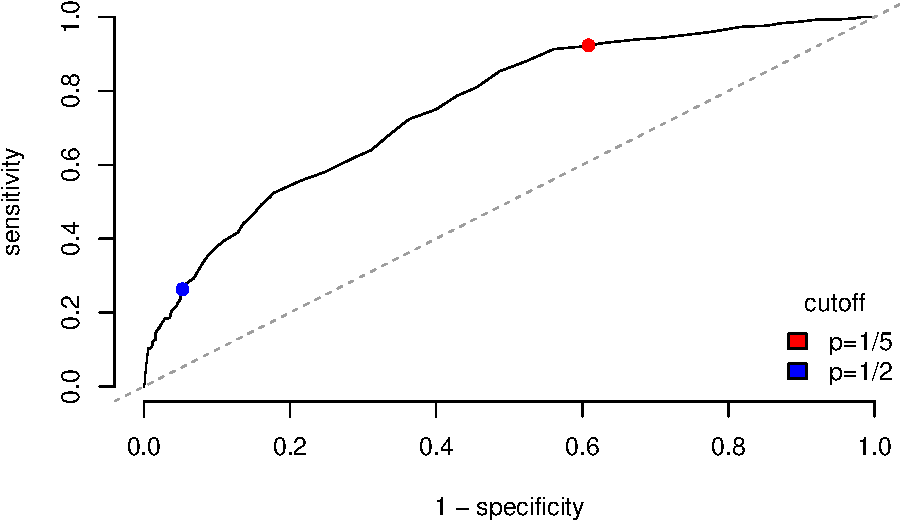
\includegraphics[scale=0.4]{figures/roc}                            
 \end{figure}

\end{column}
\end{columns}


\end{frame}
%----------------------------------------------------------------------%
\begin{frame}[fragile]
\frametitle{ROC}



\begin{columns}[T] % align columns
\begin{column}{.52\textwidth}
\begin{itemize}
\item ROC ilustra el trade-off de las reglas de clasificación
\medskip
\item ROC nos da el $locus $ de los $TPR$ y $FPR$ para todos los posibles $c\in[0,1]$
  \begin{itemize}
    \item {\it Sensibilidad:} Tasas de Verdaderos Positivos
    \item {\it 1-Especificidad:} Tasa de Falsos Positivos
    
  \end{itemize}
\item Nos da la habilidad
\begin{itemize}
  \item Medir la capacidad predictiva del modelo
  \medskip
  \item Comparar entre modelos
  
\end{itemize}
\end{itemize}
\end{column}  
\hfill
\begin{column}{.48\textwidth}

 \begin{figure}[H] \centering
            \captionsetup{justification=centering}
              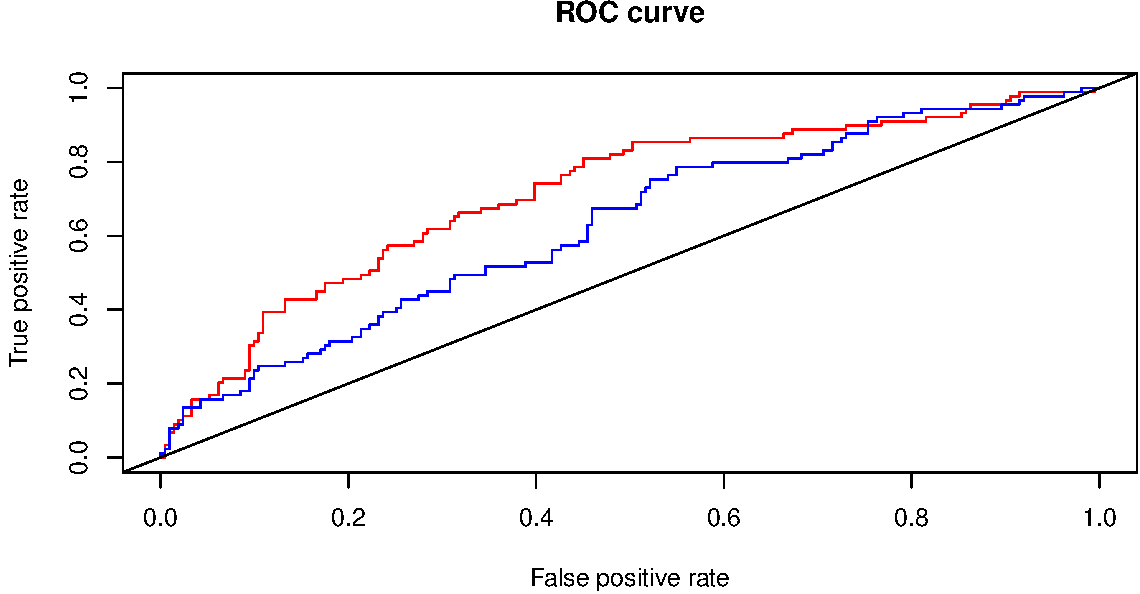
\includegraphics[scale=0.38]{figures/unnamed-chunk-11-1.pdf}
 \end{figure}

\end{column}
\end{columns}



\end{frame}


%----------------------------------------------------------------------%
\section{Más allá de la linealidad}
%----------------------------------------------------------------------%

\begin{frame}[fragile]
\frametitle{}


\centering
{\huge \textcolor{andesred}{Más allá de la linealidad}}



\end{frame}
%----------------------------------------------------------------------%
\begin{frame}
\frametitle{Más allá de la linealidad}


    \begin{itemize}
      \item El objetivo es predecir $Y$ dadas otras variables $X$. Ej: precio carros dadas caracteristicas, default, etc.
      \bigskip
      \item Asumimos que el link entre $Y$ and $X$ esta dado por el modelo:

        \bigskip
        \begin{align}
          Y = f(X) + u
        \end{align}

    \item Hasta ahora vimos modelos lineables o linealizables.
    \begin{itemize}
      \item Regresión lineal, logistica
    \end{itemize}


  \item Árboles (CARTs) 
  \begin{itemize}
    \item Modelo flexible e interpretable para la relación entre Y y X.
    \item Para que? No-linealidades,  interacciones.
  \end{itemize}
    
 
\end{itemize}





\end{frame}
%----------------------------------------------------------------------%
\begin{frame}[fragile]
\frametitle{Más allá de la linealidad: Motivación}

\begin{itemize}
\item Inspirados por Leo Breiman:

\medskip
{\scriptsize
{\it ``There are two cultures in the use of statistical modeling to reach conclusions from data. One assumes that the data are generated by a given stochastic data model. The other uses algorithmic models and treats the data mechanism as unknown.'' Breiman [2001b], p199.}
\medskip

{\it ``The statistical community has been committed to the almost exclusive use of data models. This commitment has led to irrelevant theory, questionable conclusions, and has kept statisticians from working on a large range of interesting current problems. Algorithmic modeling, both in theory and practice, has developed rapidly in fields outside statistics. It can be used both on large complex data sets and as a more accurate and informative alternative to data modeling on smaller data sets. If our goal as a field is to use data to solve problems, then we need to move away from exclusive dependence on data models and adopt a more diverse set of tools.'' Breiman [2001b], p199.}
}
\end{itemize}
\end{frame}
%----------------------------------------------------------------------%
\begin{frame}[fragile]
\frametitle{Árboles: que hacen?}


\begin{columns}[T] % align columns
\begin{column}{.42\textwidth}
  
\begin{enumerate}
    \footnotesize
\item Y es la variable a predecir, los insumos son $X_1$ y $X_2$
\item  Partimos el espacio $(X_1,X_2)$ en dos regiones, en base a una sola variable (particion horizontal o vertical).
\end{enumerate}


\end{column}  
\hfill
\begin{column}{.48\textwidth}

 \begin{figure}[H] \centering
            \captionsetup{justification=centering}
              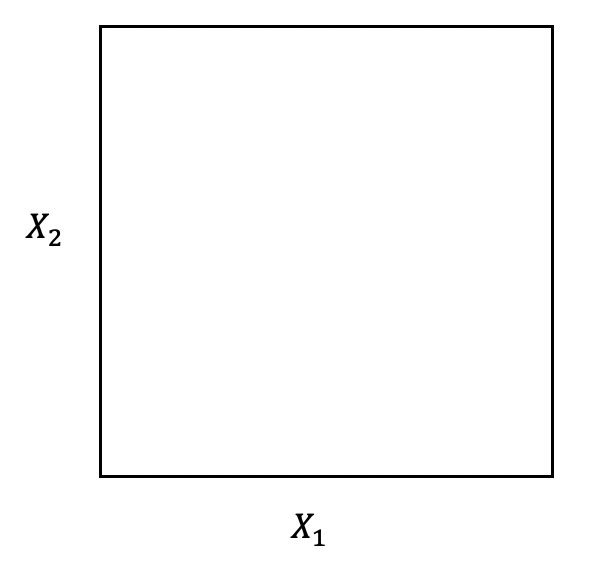
\includegraphics[scale=0.4]{figures/cart_1}                           
 \end{figure}

\end{column}
\end{columns}

\end{frame}


%----------------------------------------------------------------------%
\begin{frame}[fragile]
\frametitle{Árboles: que hacen?}


\begin{columns}[T] % align columns
\begin{column}{.42\textwidth}
  
\begin{enumerate}
    \footnotesize
\item Y es la variable a predecir, los insumos son $X_1$ y $X_2$
\item  Partimos el espacio $(X_1,X_2)$ en dos regiones, en base a una sola variable .
\item Dentro de cada región proponemos como predicción la media muestral de Y en cada región.
\item Punto: elegir la variable y el punto de partición de manera optima (mejor ajuste global).
\end{enumerate}


\end{column}  
\hfill
\begin{column}{.48\textwidth}

 \begin{figure}[H] \centering
            \captionsetup{justification=centering}
              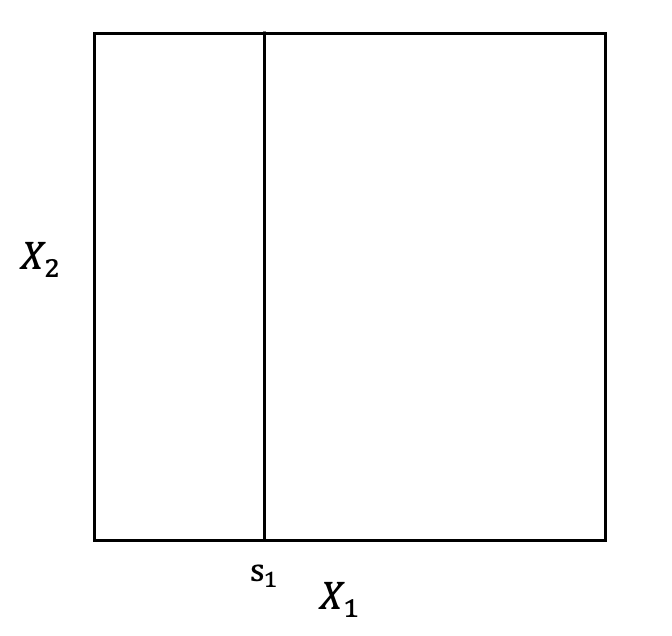
\includegraphics[scale=0.4]{figures/cart3}                           
 \end{figure}

\end{column}
\end{columns}

\end{frame}

%----------------------------------------------------------------------%
\begin{frame}[fragile]
\frametitle{Árboles: que hacen?}


\begin{columns}[T] % align columns
\begin{column}{.42\textwidth}
  
\begin{enumerate}
    \footnotesize
\item Y es la variable a predecir, los insumos son $X_1$ y $X_2$
\item  Partimos el espacio $(X_1,X_2)$ en dos regiones, en base a una sola variable .
\item Dentro de cada región proponemos como predicción la media muestral de Y en cada región.
\item Punto: elegir la variable y el punto de partición de manera optima (mejor ajuste global).
\end{enumerate}


\end{column}  
\hfill
\begin{column}{.48\textwidth}

 \begin{figure}[H] \centering
            \captionsetup{justification=centering}
              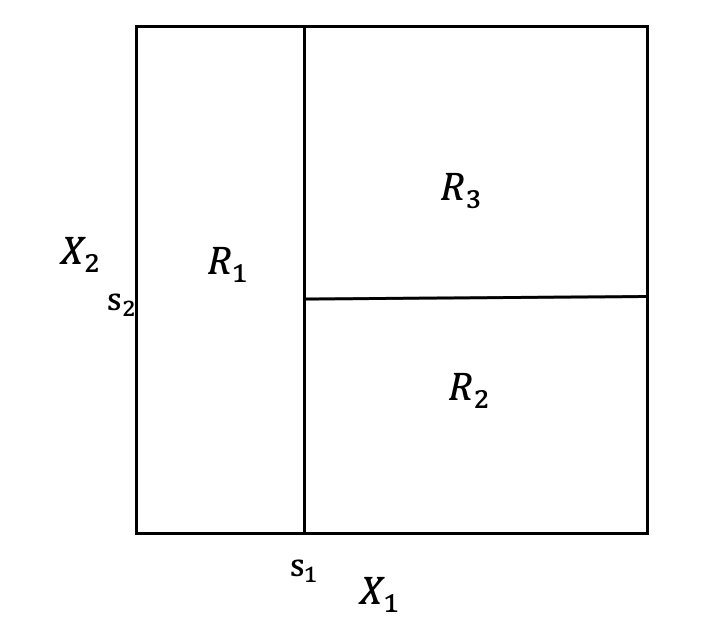
\includegraphics[scale=0.4]{figures/cart4}                           
 \end{figure}

\end{column}
\end{columns}

\end{frame}
%----------------------------------------------------------------------%
\begin{frame}[fragile]
\frametitle{Árboles: que hacen?}


\begin{columns}[T] % align columns
\begin{column}{.42\textwidth}
  
\begin{enumerate}
    \footnotesize
\item Y es la variable a predecir, los insumos son $X_1$ y $X_2$
\item  Partimos el espacio $(X_1,X_2)$ en dos regiones, en base a una sola variable (partición horizontal o vertical).
\item Dentro de cada región proponemos como predicción la media muestral de Y en cada región.
\item Punto: elegir la variable y el punto de partición de manera optima (mejor ajuste global).
\item Continuamos partiendo
\end{enumerate}


\end{column}  
\hfill
\begin{column}{.48\textwidth}

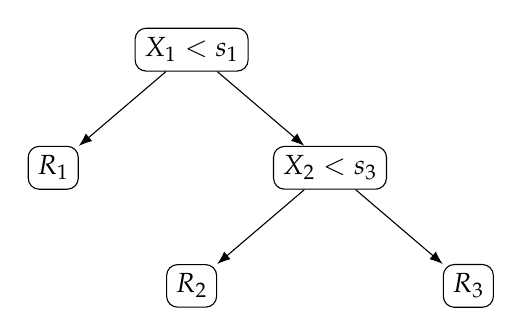
\begin{tikzpicture}[sibling distance=10em,
  every node/.style = {shape=rectangle, rounded corners,
    draw, align=center,
    top color=white, bottom color=white}]]
  \node {$X_1 < s_1$}
  child { node {$R_1$} }
    child { node {$X_2 < s_3$} 
            child{node {$R_2$}}
            child{node {$R_3$}}};
    
\end{tikzpicture}

\end{column}
\end{columns}


\end{frame}

%----------------------------------------------------------------------%
\begin{frame}[fragile]
\frametitle{Árboles: que hacen?}




  
\begin{figure}[H] \centering
            \captionsetup{justification=centering}
              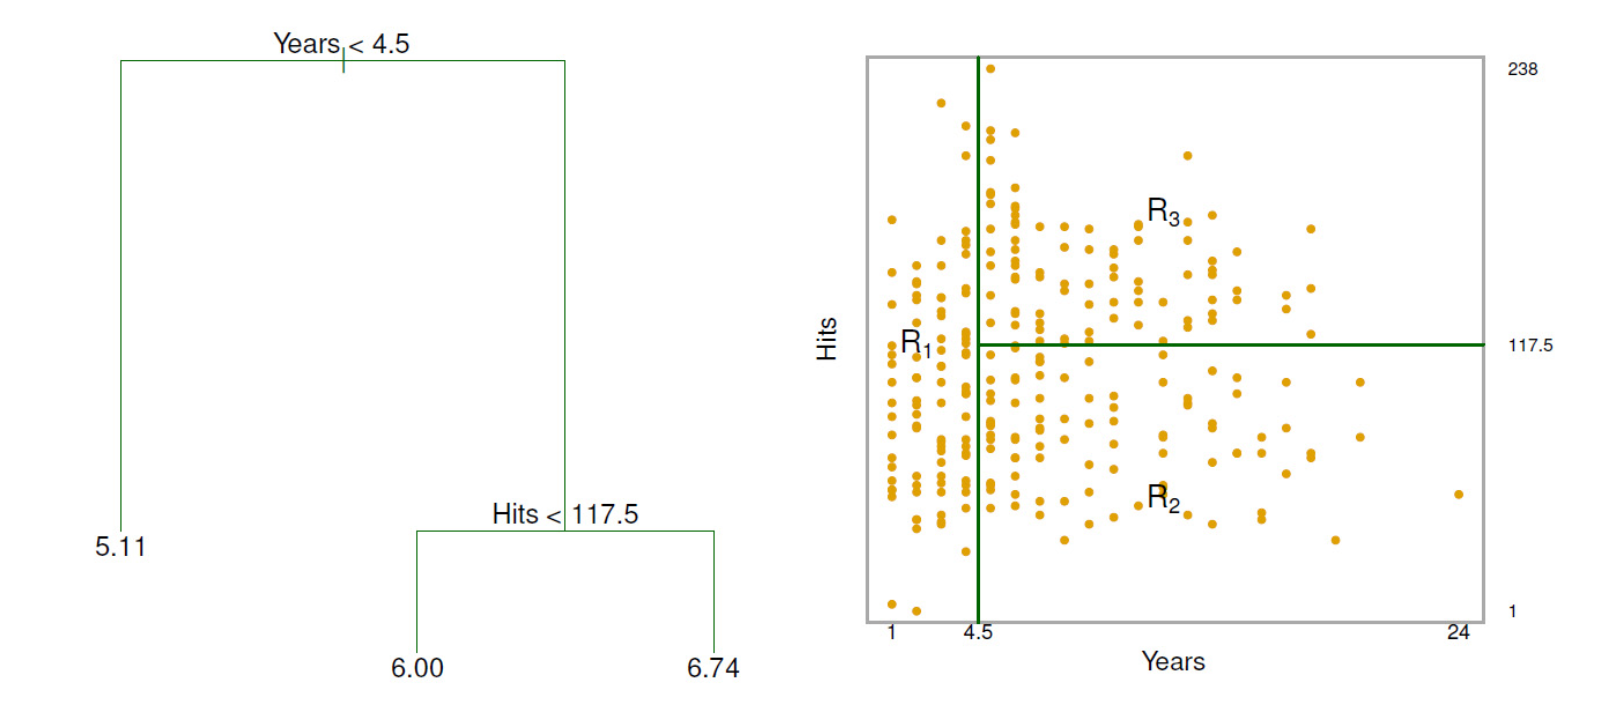
\includegraphics[scale=0.5]{figures/hitters}
 \end{figure}



\end{frame}

%----------------------------------------------------------------------%
\begin{frame}[fragile]
\frametitle{Árboles: cómo lo hacen?}

\begin{itemize}
\item Tenemos datos $y_{n\times 1}$ (precio) y $X_{n\times p}$ (características)
\item Definiciones
\begin{itemize}
\item $j$ es la variable que parte el espacio y  $s$ es el punto de partición
\item Defina los siguientes semiplanos
\begin{align}
R_1(j,s)=\{X|X_j\leq s\} \,\,\, \& \,\,\, R_2(j,s)=\{X|X_j > s\}
\end{align}
\item El problema se reduce a buscar la variable de partición $X_j$ y el punto $s$ de forma tal que 
\begin{align}
\underset{j,s}{min} \left[ \underset{c_1}{min}\sum_{x_i\in R_1(j,s)}(y-c_1)^2+ \underset{c_2}{min}\sum_{x_i\in R_2(j,s)}(y-c_2)^2\right]
\end{align}
\end{itemize}
\end{itemize}
\end{frame}
%----------------------------------------------------------------------%
\begin{frame}<1>[label=how]
\frametitle{Árboles: cómo lo hacen?}

\begin{itemize}
\item Para cada variable y punto, la minimización interna es la media
\begin{align}
 \hat{c}_m =\frac{1}{n_m} \sum(y_i|x_i \in R_m)
\end{align}
\item El proceso se repite para todas las regiones
\pause
\item El árbol final tiene M regiones
\begin{align}
\hat{f}(x) = \sum_{m=1}^M \hat{c}_m I(x \in R_m)
\end{align}

\end{itemize}

\end{frame}

%----------------------------------------------------------------------%
%----------------------------------------------------------------------%
\againframe<2>{how}

%----------------------------------------------------------------------%
\begin{frame}[fragile]
\frametitle{Árboles: cómo lo hacen?}
\begin{itemize}
\item El árbol creció, como lo paramos?
\medskip
\item Si el árbol es muy grade, tenemos overfit 
\medskip
\item Un árbol mas chico, puede tener menos regiones. Esto puede llevar a una varianza menor y mejor interpretación al costo de un poco sesgo.
\medskip
\item Solución: Pruning (poda)
\begin{itemize}
 \item Dejar crecer un árbol muy grande $T_0$
 \item Cortarlo te quedas con un sub-árbol ({\it subtree})
 \item Como determinamos la mejor forma de cortarlo? $\rightarrow$ menor error de predicción usando cross-validation
\end{itemize}

\end{itemize}

\end{frame}
%----------------------------------------------------------------------%
\begin{frame}[fragile]
\frametitle{Árboles: cómo lo hacen?}

\begin{itemize}
\item Desventaja, calcular el error de predicción usando cross-validation para cada sub-árbol posible es demasiado (muchos sub-árboles posbiles)
\medskip
\item Solución: {\it Cost complexity pruning (cortar las ramas mas débiles)}
\medskip
\begin{itemize}
    \item Indexamos los arboles con  $T$.
    \medskip
    \item Un sub-árbol $T \in T_0$ es un árbol que se obtuvo colapsando los nodos terminales de otro árbol (cortando ramas).
    \medskip
    \item  $[T]$ = número de nodos terminales del arbol  $T$
\end{itemize}
\end{itemize}
\end{frame}
%----------------------------------------------------------------------%
\begin{frame}[fragile]
\frametitle{Árboles: cómo lo hacen?}

\begin{itemize}
\item Cost complexity del árbol  $T$
\begin{align}
  C_{\alpha}(T)= \sum_{m=1}^{[T]} n_m Q_m (T) + \alpha [T]
\end{align}

  \begin{itemize}
  \item donde $Q_m (T)=\frac{1}{n_m} \sum_{x_i\in R_m} (y_i-\hat{c}_m)^2$ para los árboles de regresión
  \medskip
  \item  $Q_m (T)$ penaliza la heterogeneidad dentro de la regresión y el número de regiones 
  \medskip
  \item  Objetivo: para un dado $\alpha$, encontrar el pruning óptimo que minimice  $C_{\alpha}(T)$
  \end{itemize}
\end{itemize}
\end{frame}

%----------------------------------------------------------------------%
\begin{frame}[fragile]
\frametitle{Árboles: cómo lo hacen?}

\begin{itemize}
  \item Mecanismo de búsqueda para $T_\alpha$ ( pruning óptimo dado  $\alpha$).


    \begin{quote}
    \centering
    Resultado: para cada  $\alpha$ hay un sub-árbol único  $T_\alpha$ que minimiza  C$\alpha$ (T).
    \end{quote}

\begin{itemize}

\medskip
\item Vamos a eliminar sucesivamente las ramas que producen un aumento mínimo en  $\sum_{m=1}^{[T]} n_m  Q_m (T)$
\medskip
\item Donde remover ramas es colapsar, esto aumenta la heterogenidad, ergo, colapsamos las particiones menos necesarias.
\medskip
\item Esto eventualmente colapsa hasta el nodo inicial (stump) pero va a través de una sucesión de árboles, que va del mas grande al mas pequeño cortando las ramas mas débiles.
\end{itemize}
\medskip
\item Breiman et al. (1984): $T_\alpha$ pertenece a esta sequencia. 
\medskip
\item Uno puede enfocar la búsqueda en esta sucesión de sub-árboles.
\medskip
\item Elección de $\alpha$: cross validation.


\end{itemize}




\end{frame}
%----------------------------------------------------------------------%
\begin{frame}[fragile]
\frametitle{Árboles vs. Modelos Lineales}
\begin{itemize}
\item Cuál modelo es mejor?

\begin{itemize}
  \item Si la relación entre los predictores y la respuesta es lineal, los modelos lineales clásicos, como la regresión lineal, superan a los árboles de regresión. 
  \item Por otro lado, si la relación entre los predictores no es lineal, los árboles de decisión superarían a los enfoques clásicos.
\end{itemize}
\end{itemize}


\begin{columns}[T] % align columns
\begin{column}{.42\textwidth}
\scriptsize
\begin{itemize}  
\item Arriba: el límite es lineal
  \begin{itemize}
    \scriptsize
    \item Izquierda:  modelo lineal (bueno)
    \item Derecha: árbol 
  \end{itemize}

\item Abajo: el límite es no-lineal
  \begin{itemize}
    \scriptsize
    \item Izquierda: linear model 
    \item Derecha: arbol (good)
  \end{itemize}

\end{itemize}


\end{column}  
\hfill
\begin{column}{.48\textwidth}

 \begin{figure}[H] \centering
            \captionsetup{justification=centering}
              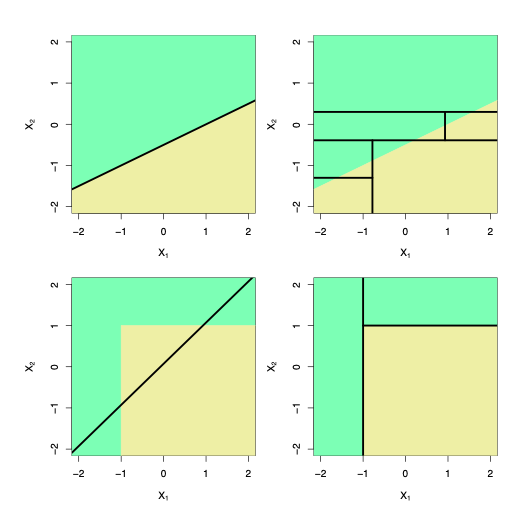
\includegraphics[scale=0.55]{figures/tree_vs_reg}
 \end{figure}

\end{column}
\end{columns}




\end{frame}

%----------------------------------------------------------------------%
\begin{frame}[fragile]
\frametitle{Ventajas y Desventajas de los Árboles}

\begin{itemize}
\item Pros: 
  \begin{itemize}
    \item Los árboles son muy fáciles de explicar a las personas (probablemente incluso más fáciles que la regresión lineal)
    \medskip
    \item Los árboles se pueden trazar gráficamente y son fácilmente interpretados incluso por no expertos. Variables más importantes en la parte superior
    \medskip
    \item Funcionan bien en problemas de clasificación y regresión.
  \end{itemize}

\bigskip
\item  Cons:
  \begin{itemize}
    \item Los árboles no son muy precisos o robustos (ensamblados, bosques aleatorios y boosting al rescate)
    \medskip
    \item Si la estructura es lineal, CART no funciona bien
  \end{itemize}
\end{itemize}

\end{frame}

%----------------------------------------------------------------------%
\section{Bagging and Random Forests }
%----------------------------------------------------------------------%
\begin{frame}[fragile]
\frametitle{Bagging}

\begin{itemize}
  \item Problema con CART: varianza alta.
  \medskip
   \item Podemos mejorar mucho el rendimiento mediante la agregación 
   \medskip
   \item Bagging:
    \begin{itemize}
       \item Obtenga repetidamente muestras aleatorias $(X_i^b,Y_i^b)_{i=1}^N$ de la muestra observada.
       \medskip
       \item Para cada muestra de arranque, ajuste un árbol de regresión $\hat{f}^b(x)$
       \medskip
       \item Promedie las muestras de bootstrap 
        \begin{align}
         \hat{f}_{bag} =\frac{1}{B}\sum_{b=1}^B \hat{f}^b(x)
        \end{align}
      \end{itemize}
  \item Básicamente estamos suavizando las predicciones.
  \medskip
  \item Idea: la varianza del promedio es menor que la de una sola predicción.
  \end{itemize}

\end{frame}

%----------------------------------------------------------------------%
\begin{frame}[fragile]
\frametitle{Random Forests}

\begin{itemize}
  \item Problema con el bagging: si hay un predictor fuerte, diferentes árboles son muy similares entre sí. Si hay alta correlación, ¿está realmente reduciendo la varianza?
\bigskip
\item Bosques (forests): reduzca la correlación entre los árboles  en el boostrap.
\bigskip
\item Si hay $p$ predictores, en cada partición use solo  $m <p$ predictores, elegidos al azar.
\bigskip
\item Bagging es forests con $m = p$ (usando todo los predictores en cada partición).
\bigskip
\item Tipicamente $m = \sqrt(p)$
\end{itemize}

\end{frame}

%----------------------------------------------------------------------%
\begin{frame}[fragile]
\frametitle{Random Forests}

\begin{figure}[H] \centering
            \captionsetup{justification=centering}
              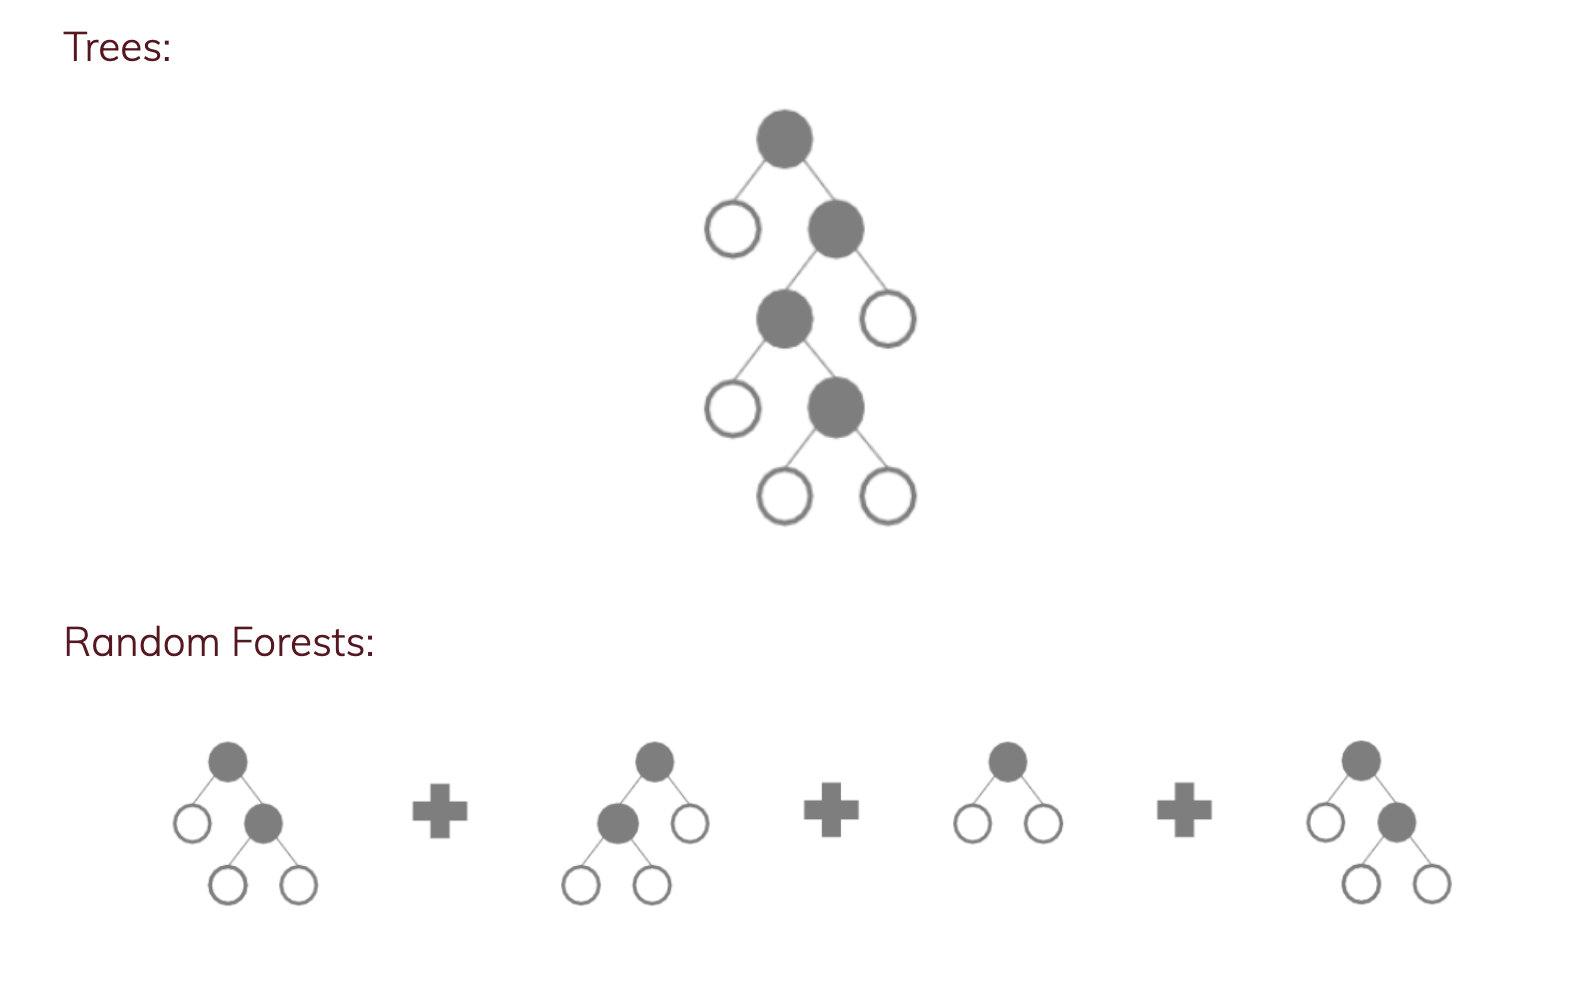
\includegraphics[scale=0.4]{figures/trees_to_forests.png}
 \end{figure}
\end{frame}

%----------------------------------------------------------------------%
\begin{frame}[fragile]
\frametitle{Random Forests}

\begin{figure}[H] \centering
            \captionsetup{justification=centering}
              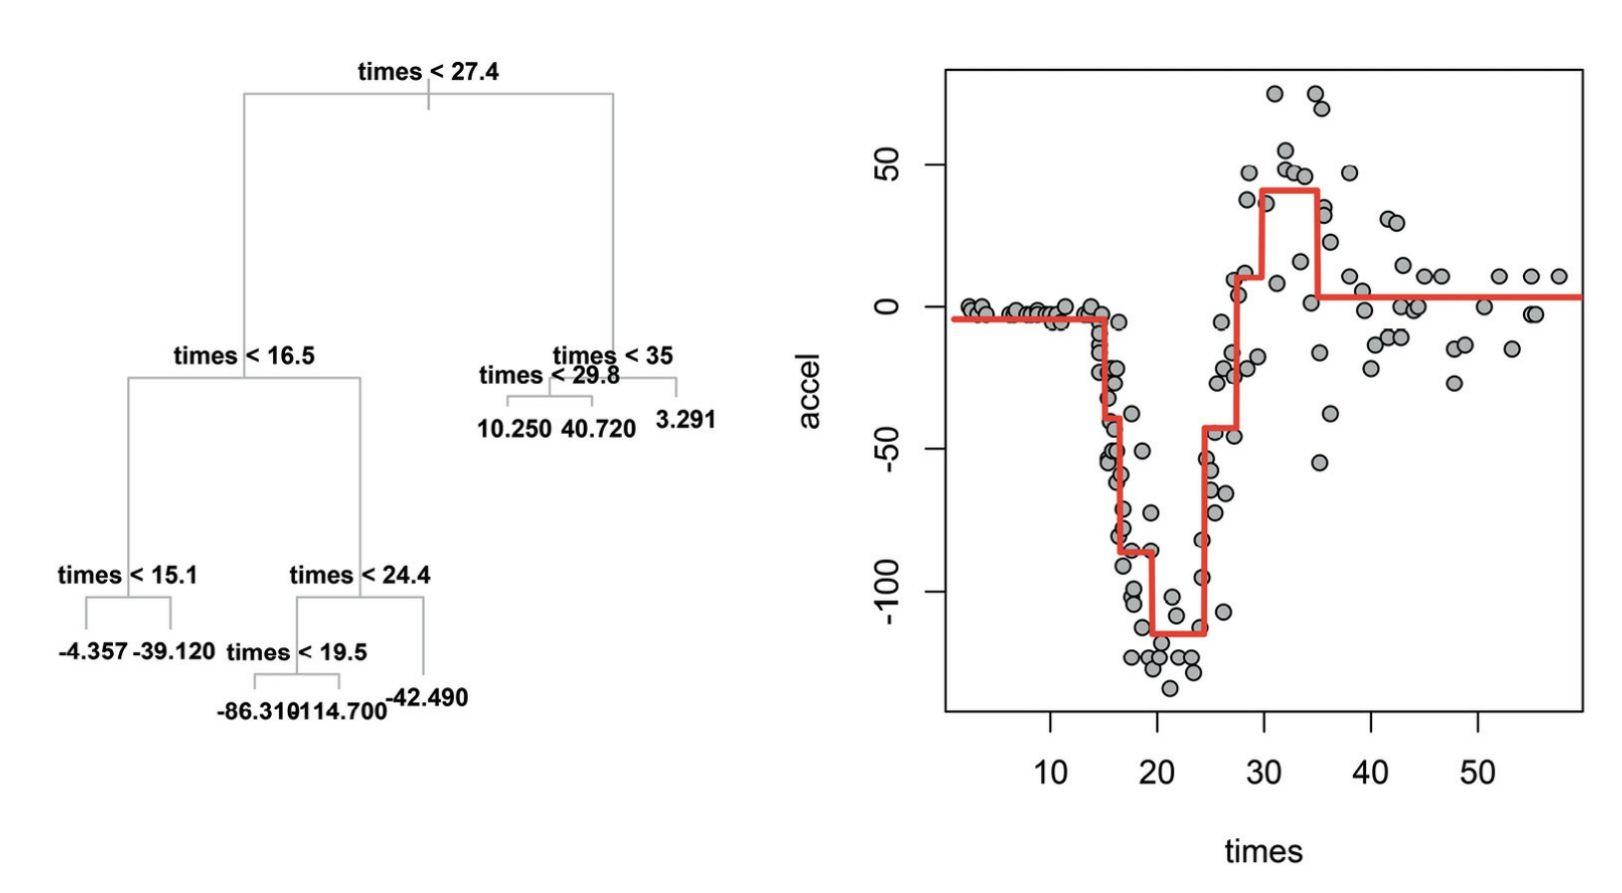
\includegraphics[scale=0.25]{figures/accel_1}
 \end{figure}
\end{frame}

%----------------------------------------------------------------------%
\begin{frame}[fragile]
\frametitle{Random Forests}

\begin{figure}[H] \centering
            \captionsetup{justification=centering}
              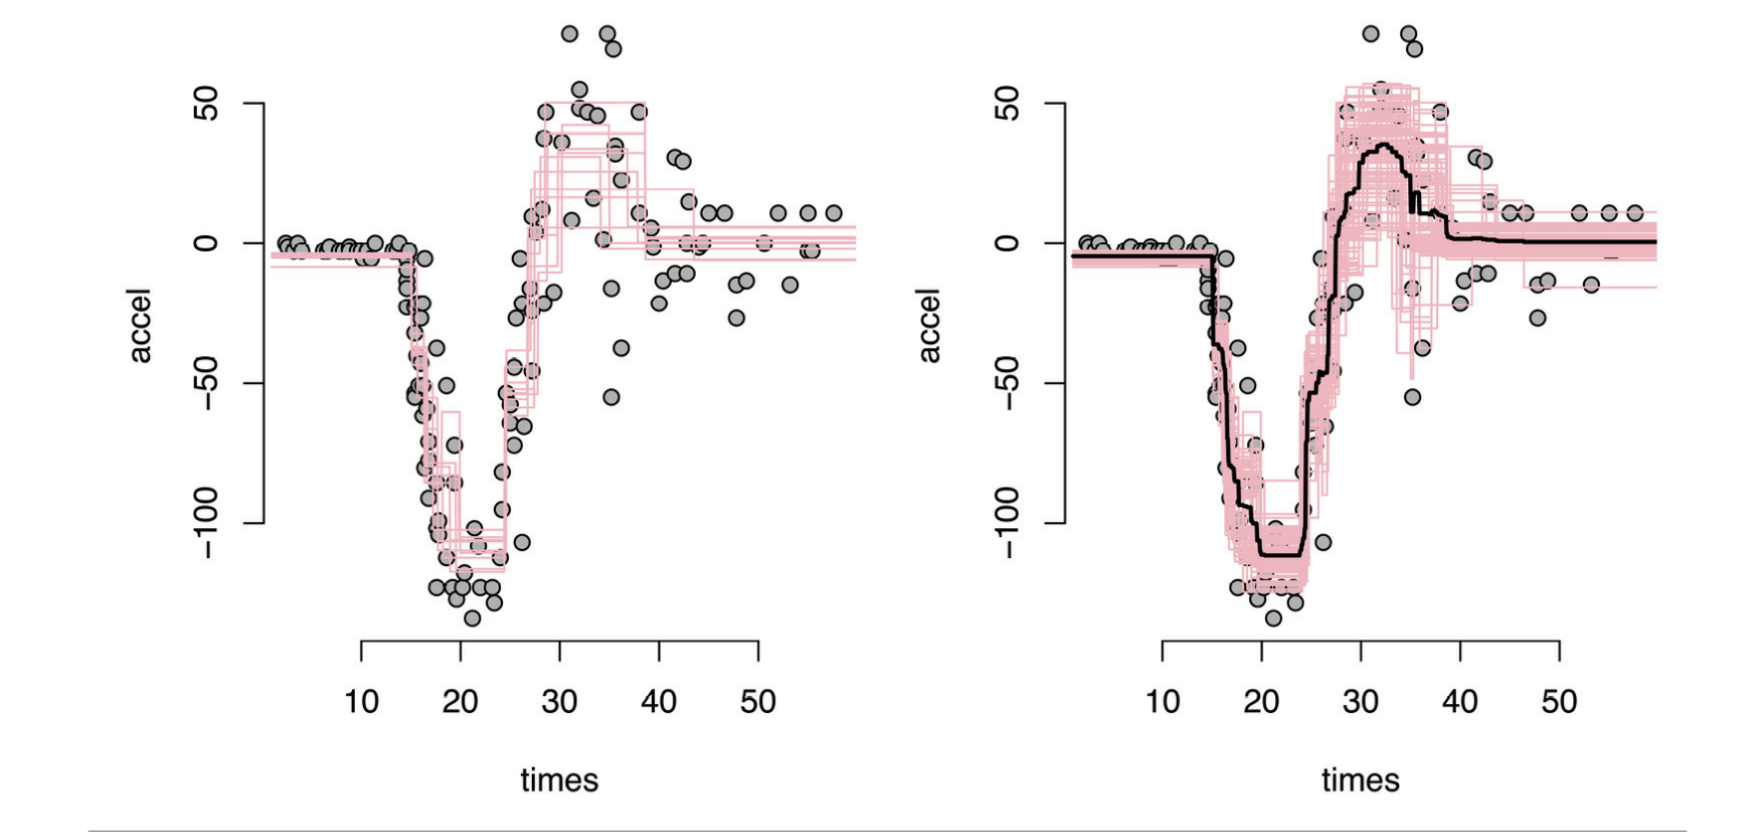
\includegraphics[scale=0.25]{figures/accel_2}
 \end{figure}
\end{frame}

%----------------------------------------------------------------------%
\begin{frame}[fragile]
\frametitle{Random Forests}

\begin{figure}[H] \centering
            \captionsetup{justification=centering}
              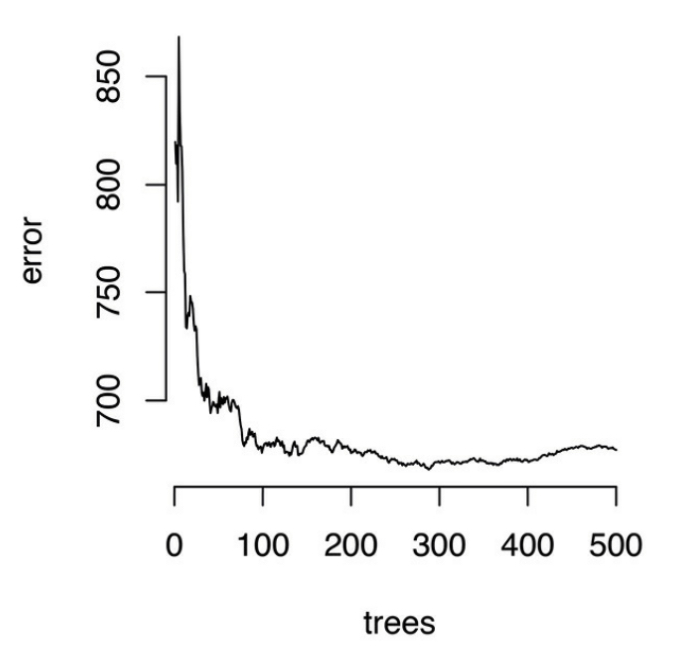
\includegraphics[scale=0.25]{figures/accel_3}
 \end{figure}
\end{frame}

%----------------------------------------------------------------------%
\subsection{Comparación: Árboles y Bosques}
%----------------------------------------------------------------------%

%----------------------------------------------------------------------%
\begin{frame}[fragile]
\frametitle{Comparación: Árboles y Bosques}
\frametitle{ MSE Fuera de Muestra}


\begin{figure}[H] \centering
            \captionsetup{justification=centering}
              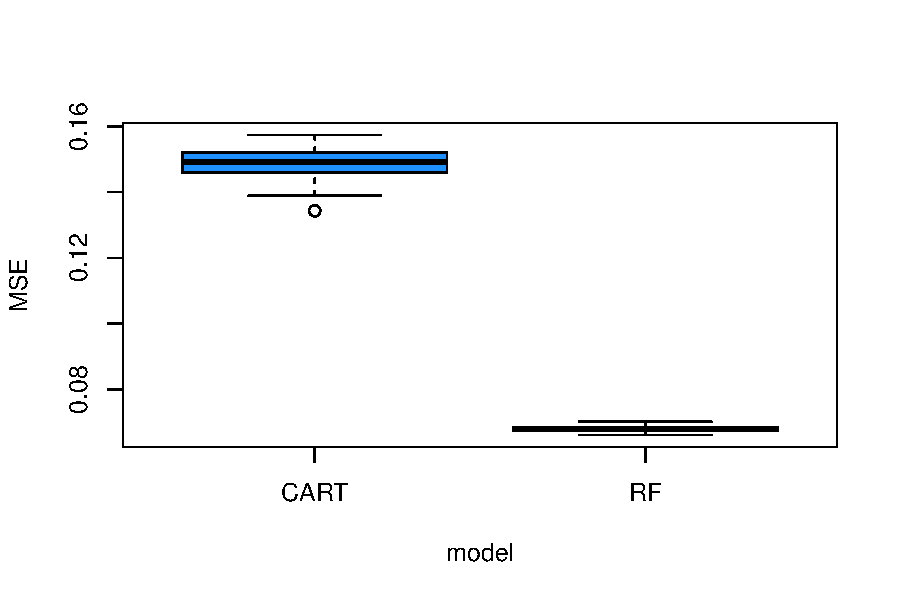
\includegraphics[scale=.75]{figures/mse_tree.pdf}
 \end{figure}

\end{frame}


%----------------------------------------------------------------------%
\section{Boosting}
\subsection{Motivation}
%----------------------------------------------------------------------%
\begin{frame}[fragile]
\frametitle{Boosting: Motivation}

\begin{itemize}
  \item Problema con CART: varianza alta.
  \medskip
   \item Podemos mejorar mucho el rendimiento mediante la agregación 
   \medskip 
   \item El boosting toma esta idea pero lo "encara" de una manera diferente $\rightarrow$ viene de la computación
   \medskip
   \item Va a usar clasificadores débiles: clasificador marginalmente mejor que lanzar una moneda (tasa de error ligeramente mejor que .5) 
\medskip
\item Ej.: CART con pocas ramas (dos ramas) 
\medskip
\item Boosting: promedio ponderado de la sucesión de clasificadores débiles.

\end{itemize}
\end{frame}
%----------------------------------------------------------------------%
\begin{frame}[fragile]
\frametitle{Boosting}

\begin{itemize}
  \item El boosting viene de la computación y tiene un lenguaje ligeramente diferente.
  \medskip
  \item Fue desarrollado para problemas de clasificación pero se puede extender fácilmente a regresión.
\medskip
\item Vocabulario:
\medskip
  \begin{itemize}
  \item $y \in {-1,1}$, $X$ vector de predictores.
  \medskip
  \item $y = G (X)$ (clasificador)
  \medskip
  \item $err = \frac{1}{N} \sum_{i}^N I(y_i\neq G(x_i))$
  \end{itemize}
  \medskip
  \item Para fijar ideas veamos \texttt{AdaBoost}
\end{itemize}


\end{frame}

%----------------------------------------------------------------------%
\subsection{AdaBoost}
%----------------------------------------------------------------------%
\begin{frame}[fragile]
\frametitle{AdaBoost}
\begin{enumerate}
\item Comenzamos con ponderadores $w_i = 1 / N$
\item Para m = 1 hasta M:
\begin{enumerate}
    \item Estimar $G_m(x)$ usando ponderadores $w_i$ .
    \item Computar el error de predicción
    \begin{align}
    err_m = \frac{\sum_{i=1}^N  I(y_i \neq G_m(x_i))}{\sum_{i=1}^N w_i}
    \end{align}
    \item Obtener $\alpha_m= ln \left[\frac{(1 - err m )}{ err m} \right]$
    \item Actualizar los ponderadores : $w_i \leftarrow w_i c_i$ 
    \begin{align}
    c_i = exp \left[\alpha_m  I (y i \neq G_m (x_i )) \right]
    \end{align}
    
\end{enumerate}
\item Resultado: $G(x) = sgn[\sum_{m = 1}^M \alpha_m G_m(x)]$
\end{enumerate}

\end{frame} 
%----------------------------------------------------------------------%
\begin{frame}[fragile]
\frametitle{AdaBoost}

\begin{itemize}
\item $c_i = exp \left[ \alpha_m I(y_i \neq G_m (x_i )) \right]$
\medskip
\item Si fue correctamente predicho, $c_i = 1$. 
\medskip
\item En caso contrario, $c_i = exp (\alpha_m ) = \frac{(1 - err_m ) }{err_m} > 1$ 
\medskip
\item En cada paso el algoritmo da mas importancia relativa a las predicciones incorrectas.
\medskip
\item Paso final: promedio ponderado de estos pasos
\end{itemize}
\begin{align}
G(x) = sgn[\sum_{m = 1}^M \alpha_m G_m(x)]
\end{align}

\end{frame}
%----------------------------------------------------------------------%
\begin{frame}[fragile]
\frametitle{Boosting Intuición}


\begin{figure}[H] \centering
            \captionsetup{justification=centering}
              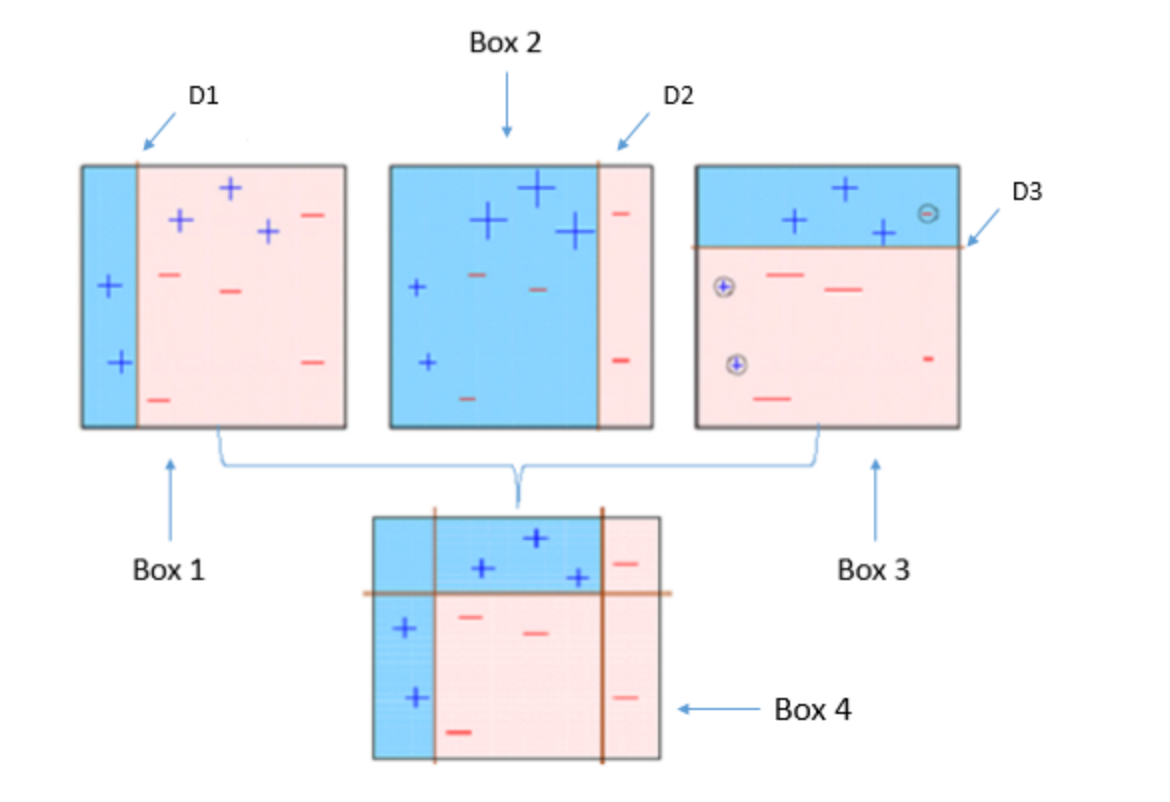
\includegraphics[scale=0.5]{figures/adaboost.png}
              \\
              \tiny
              Source: \url{https://www.analyticsvidhya.com/blog/2015/11/quick-introduction-boosting-algorithms-machine-learning/}
 \end{figure}

\end{frame}

%----------------------------------------------------------------------%
\subsection{Boosting Trees}
 %----------------------------------------------------------------------%
%----------------------------------------------------------------------%
\begin{frame}[fragile]
\frametitle{Boosting Trees: Algoritmo}

\begin{itemize}
\item En el caso de los árboles ($\hat{f}(x)$) aprender su estructura es mucho mas difícil. 
\medskip
\begin{itemize}
  \item Necesitamos saber el tamaño del árbol.
  \medskip 
  \item Es intratable aprender todos los arboles al mismo tiempo.
  \medskip
\end{itemize}
  \item La estrategia de boosting es aprender iterativamente.
  \medskip 
  \item Fijamos lo aprendido, y agregamos un nuevo árbol en cada paso.
  \medskip
  \item Escribimos el valor de la predicción en cada paso $m$ como  $\hat{y}_i^{m}$. 
\end{itemize}
\end{frame}
%----------------------------------------------------------------------%
\begin{frame}[fragile]
\frametitle{Boosting Trees: Algoritmo}
\begin{itemize}
\item La estrategia de boosting es aprender iterativamente.
\medskip
\item Fijamos lo aprendido, y agregamos un nuevo árbol en cada paso.
\medskip
\item Escribimos el valor de la predicción en cada paso $m$ como  $\hat{y}_i^{m}$. 
\medskip
\item Entonces tenemos
\begin{align}
\hat{y}_i^{0} &=0 \\ \nonumber
\hat{y}_i^{1} &= \hat{y}_i^{0} + f_1(x_i) \\ \nonumber
\hat{y}_i^{2} &= \hat{y}_i^{1} + f_2(x_i) \\ \nonumber
\dots \\ \nonumber
\hat{y}_i^{M} &= \sum_{m=1}^M f_m(x_i) = \hat{y}_i^{m-1} + f_m(x_i) \\ \nonumber
\end{align}
\end{itemize}


 \end{frame}
%----------------------------------------------------------------------%
\begin{frame}[fragile]
\frametitle{Boosting Trees: Algoritmo}

\begin{itemize}


\item ¿Qué árbol agregamos en cada paso?
\item El que optimice el objetivo

\begin{align}
obj^m &= \sum_{i=1}^N L(y_i,\hat{y}_i^{(m)}) \\
     &= \sum_{i=1}^N L(y_i,\hat{y}_i^{m-1} + f_m(x_i))
\end{align}

\item Si usamos MSE como $L$ la función objetivo es

\begin{align}
\sum_{i=1}^N (y_i-\hat{y}_i^{m-1} + f_m(x_i))^2
\end{align}

\end{itemize}
\end{frame}
%----------------------------------------------------------------------%
\begin{frame}[fragile]
\frametitle{Boosting Trees: Iteraciones}

\begin{itemize}

\item La pregunta se vuelve cuantas iteraciones (M) usar?
\begin{itemize}
\medskip
  
  \item Cada iteración generalmente reduce el riesgo de entrenamiento $L (.)$, de modo que para M lo suficientemente grande este riesgo puede hacerse arbitrariamente pequeño (sesgo se va a cero).
  \medskip
  \item Sin embargo, ajustar demasiado bien los datos de entrenamiento puede llevar a overfit (sobreajuste)
  \medskip
  \item Por lo tanto, hay un número óptimo $ M^\star$ que minimiza el error fuera de muestra
  \medskip
  \item Una forma conveniente de estimar $ M^\star$ es calcular el error de predicción como una función de M en una muestra de validación. El valor de M que minimiza este riesgo se toma como una estimación de M. 

  \end{itemize}
\end{itemize}
\end{frame}


%----------------------------------------------------------------------%
\subsection{Boosting Trees: Demo} 
%----------------------------------------------------------------------%
\begin{frame}[fragile]
\frametitle{Boosting Trees: Demo}
\begin{figure}[H] \centering
            \captionsetup{justification=centering}
              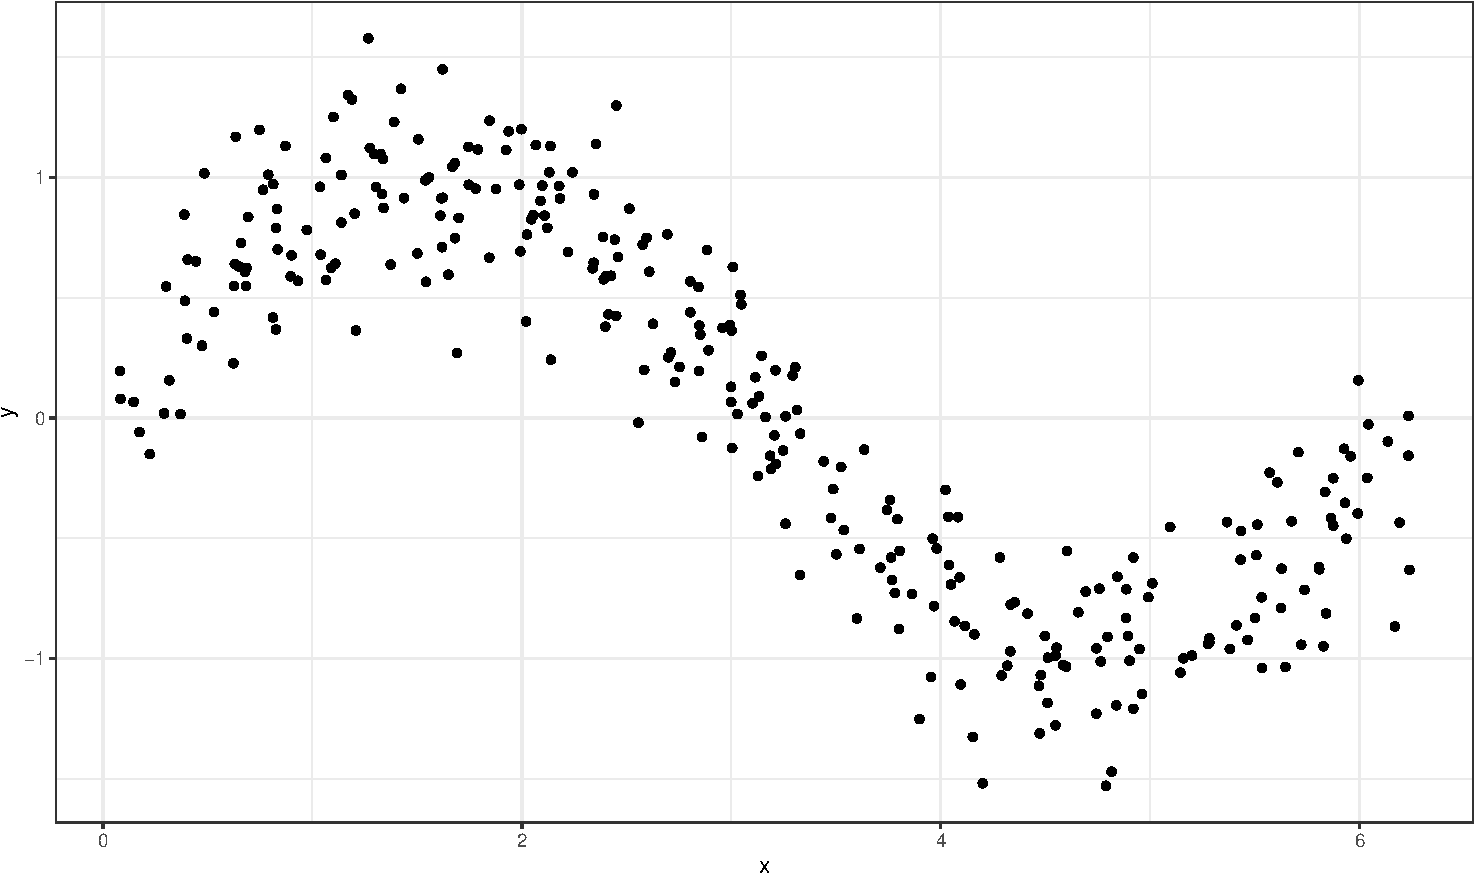
\includegraphics[scale=0.5]{figures/unnamed-chunk-3-1.pdf}
 \end{figure}


 \end{frame}
%----------------------------------------------------------------------%
\begin{frame}[fragile]
\frametitle{Boosting Trees: Example}

\begin{itemize}
\item Algorithm:
\end{itemize}

\begin{Shaded}
\begin{Highlighting}[]
\NormalTok{M\textless{}{-}}\DecValTok{2}
\end{Highlighting}
\end{Shaded}

\begin{figure}[H] \centering
            \captionsetup{justification=centering}
              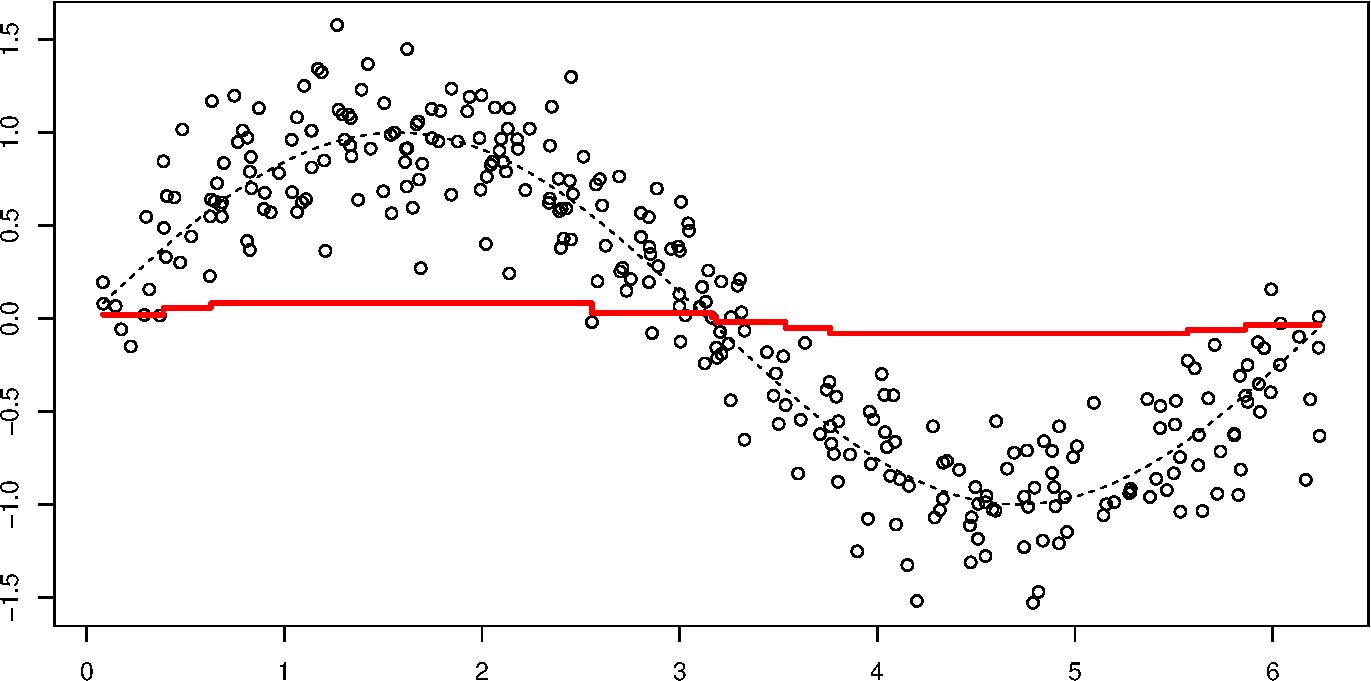
\includegraphics[scale=0.5]{figures/unnamed-chunk-5-1.pdf}
 \end{figure}

 \end{frame}
%----------------------------------------------------------------------%
\begin{frame}[fragile]
\frametitle{Boosting Trees: Example}

\begin{Shaded}
\begin{Highlighting}[]
\NormalTok{M\textless{}{-}}\DecValTok{10}
\end{Highlighting}
\end{Shaded}

\begin{figure}[H] \centering
            \captionsetup{justification=centering}
              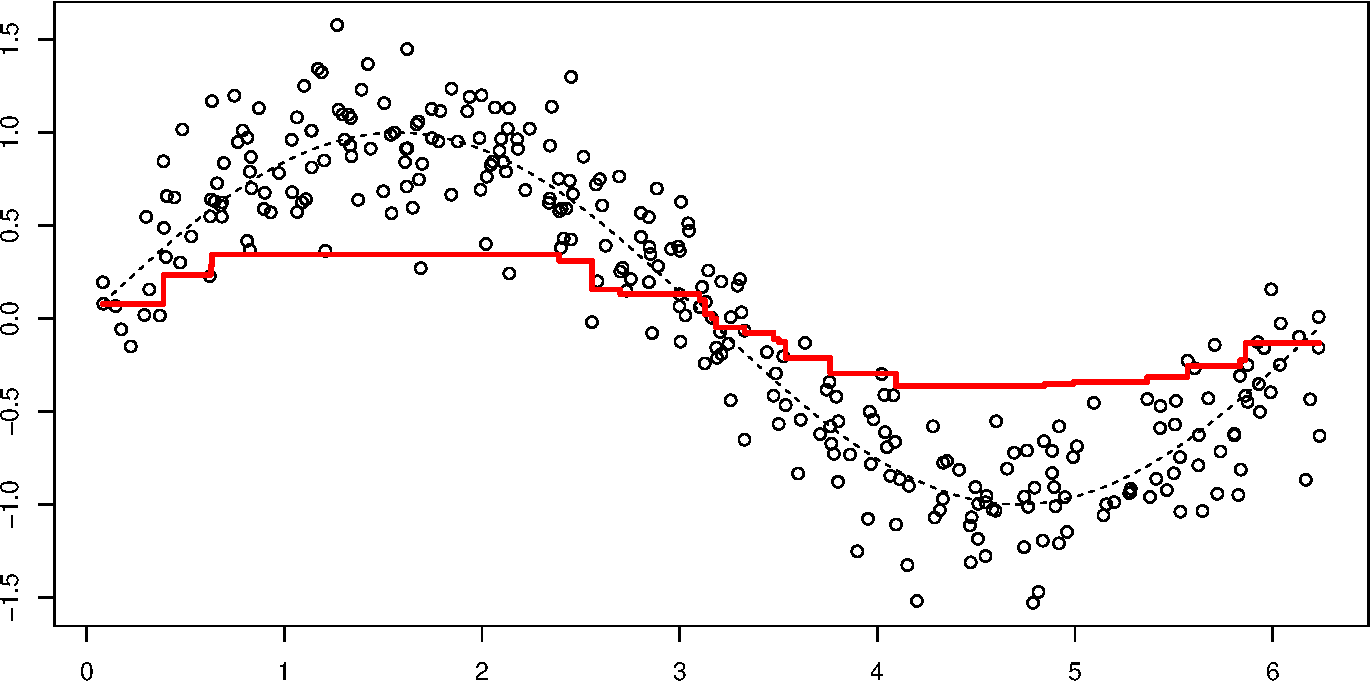
\includegraphics[scale=0.5]{figures/unnamed-chunk-6-1.pdf}
 \end{figure}
 \end{frame}
%----------------------------------------------------------------------%
\begin{frame}[fragile]
\frametitle{Boosting Trees: Example}

\begin{Shaded}
\begin{Highlighting}[]
\NormalTok{M\textless{}{-}}\DecValTok{100}
\end{Highlighting}
\end{Shaded}

\begin{figure}[H] \centering
            \captionsetup{justification=centering}
              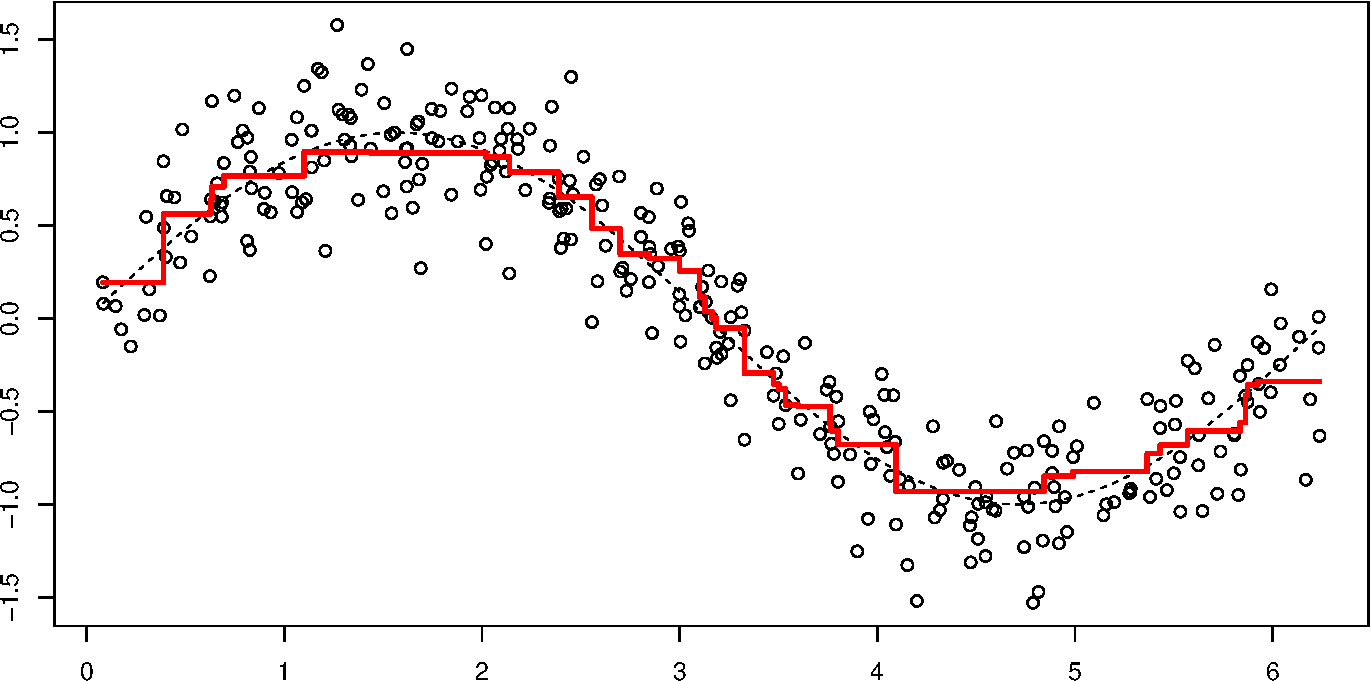
\includegraphics[scale=0.5]{figures/unnamed-chunk-7-1.pdf}
 \end{figure}

 \end{frame}
%----------------------------------------------------------------------%
\begin{frame}[fragile]
\frametitle{Boosting Trees: Example}

\begin{Shaded}
\begin{Highlighting}[]
\NormalTok{M\textless{}{-}}\DecValTok{300}

\end{Highlighting}
\end{Shaded}

\begin{figure}[H] \centering
            \captionsetup{justification=centering}
              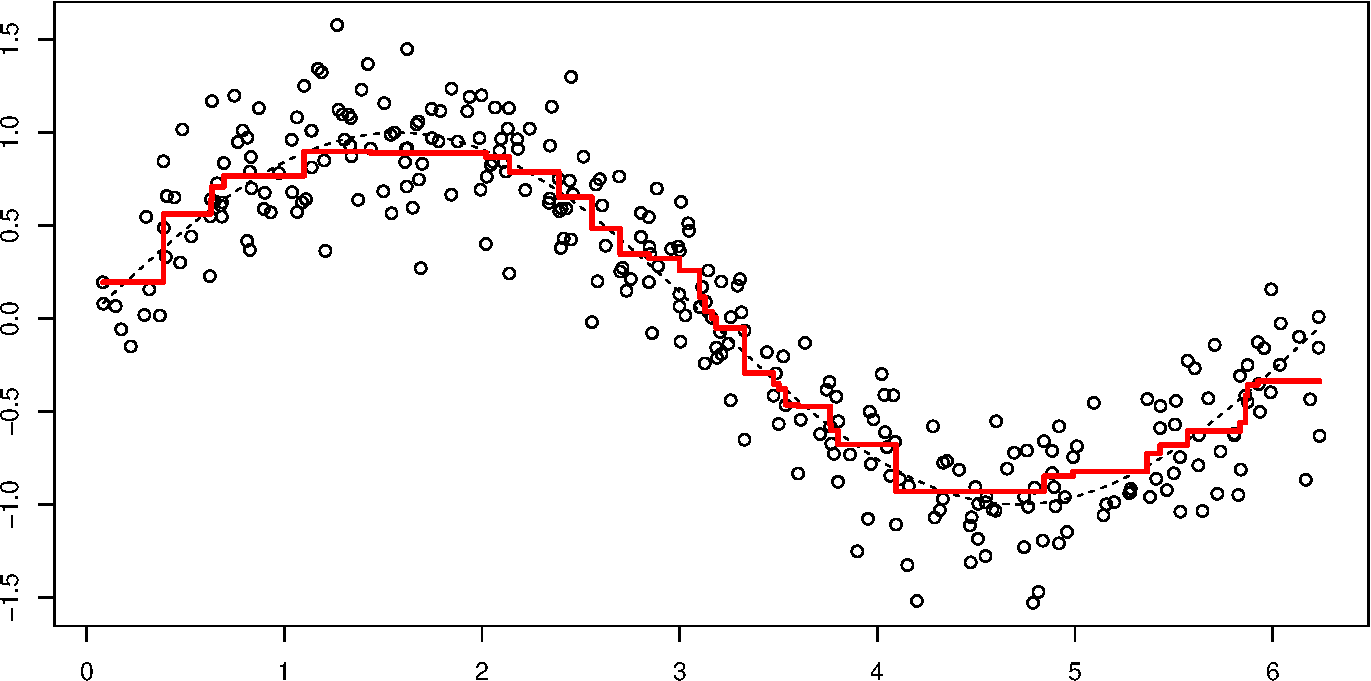
\includegraphics[scale=0.5]{figures/unnamed-chunk-8-1.pdf}
 \end{figure}

 \end{frame}
%----------------------------------------------------------------------%
\begin{frame}[fragile]
\frametitle{Boosting Trees: Example}

\begin{itemize}
\item Simple tree (blue), boosted tree (red)
\end{itemize}

\begin{figure}[H] \centering
            \captionsetup{justification=centering}
              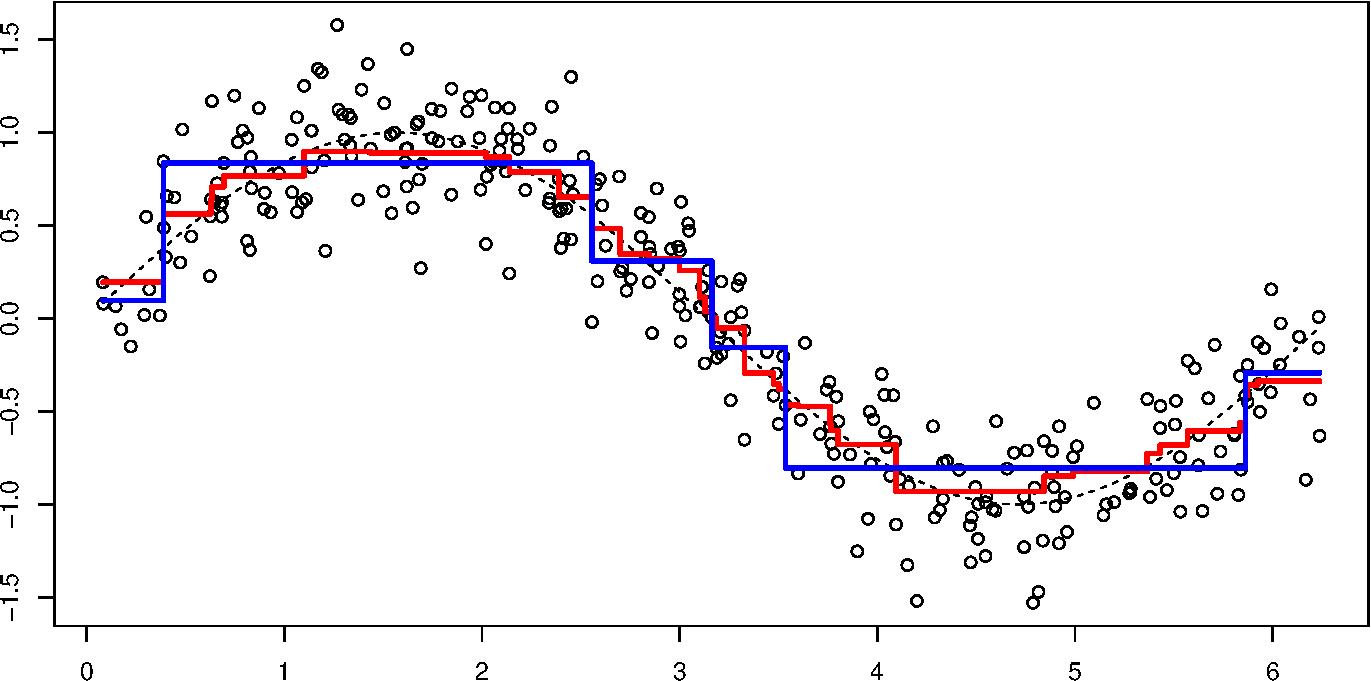
\includegraphics[scale=0.5]{figures/unnamed-chunk-9-1.pdf}
 \end{figure}

 \end{frame}
%----------------------------------------------------------------------%
\begin{frame}[fragile]
\frametitle{XGBoost en un Boosting Tree }

\begin{itemize}


\item ¿Qué árbol agregamos en cada paso?
\item El que optimice la función objetivo


\begin{align}
\mathcal{L} &= \sum_{i=1}^N L(y_i,\hat{y}_i) + \sum_{k=1}^m \Omega(f_k)
\end{align}


\item  El segundo termino penaliza la complejidad del modelo,


\begin{align}
\Omega(f)=\gamma T + \frac{1}{2}\lambda ||\omega||_2
\end{align}
\end{itemize}
\end{frame}
%----------------------------------------------------------------------%
\begin{frame}[fragile]
\frametitle{XGBoost: palabras finales}

\begin{itemize}

\item XGBoost es una extensión de boosting trees, hay muchas más.
\medskip
\item Su implementación fue diseñada específicamente para un rendimiento y velocidad óptimos.
\medskip
\item ¿Por qué hablar de XGBoost?
\begin{itemize}
\footnotesize
 \item Entre las 29 soluciones ganadoras del desafío publicadas en página de Kaggle durante 2015, 17 soluciones utilizaron XGBoost.
 \item Entre estas soluciones, ocho utilizaron exclusivamente XGBoost para entrenar el modelo, mientras que la mayoría de las demás combinaron XGBoost con redes neuronales. (El segundo método más popular, las redes neuronales profundas, se utilizó en 11 soluciones)
 \item También se vio en la competencia de Minería de Datos y Descubrimiento de Conocimiento de 2015 organizada por ACM (Copa KDD), donde XGBoost fue utilizado por todos los equipos ganadores en el top-10.
 \item Históricamente, XGBoost ha funcionado bastante bien para datos tabulares estructurados. Pero, si se trata de datos no estructurados como imágenes, las redes neuronales suelen ser una mejor opción.


\end{itemize}
 \end{itemize}
\end{frame}




%----------------------------------------------------------------------%
\section{Break}
\begin{frame}
\frametitle{}

\begin{centering}
\huge
\textcolor{andesred}{Volvemos en 15 mins con \texttt{R} }

\end{centering}

\end{frame}
%----------------------------------------------------------------------%
\section{\texttt{R para ML}}
%----------------------------------------------------------------------%
\begin{frame}
\frametitle{R para ML}

\begin{figure}[H] \centering
  \centering
  
\includegraphics[scale=0.35]{figures/baticomputer_meme.jpg}
  \\
  \tiny photo from \url{https://www.dailydot.com/parsec/batman-1966-labels-tumblr-twitter-vine/}
\end{figure}

\end{frame}
%----------------------------------------------------------------------%
%----------------------------------------------------------------------%
\end{document}
%----------------------------------------------------------------------%
%----------------------------------------------------------------------%
